%%%%%%%%%%%%%%%%%%%%%%%%%%%%%%%%%%%%%%%%%%%%%%%%%%%%%%%%%%%%%%%%%%%%%%%
%
%   TIPE OLIVIER CAFFIER MPI(*) Faidherbe
%
%%%%%%%%%%%%%%%%%%%%%%%%%%%%%%%%%%%%%%%%%%%%%%%%%%%%%%%%%%%%%%%%%%%%%%%

\documentclass{beamer}

\usetheme[hideothersubsections]{UNLTheme}
\usepackage{tikz}
\usepackage{xcolor}
\usepackage{algorithm}
\usepackage{algpseudocode}
\usepackage{listings}
\usepackage{multicol}
\usepackage[most]{tcolorbox}
\lstset{inputencoding=utf8}
\setbeamertemplate{caption}[numbered]


\usetikzlibrary{automata, positioning}
\usetikzlibrary{shapes}


\definecolor{marine_blue}{RGB}{3, 4, 94}
\lstset{
    framerule=1pt,
    frame=tb,
    emphstyle={\small\ttfamily\bfseries\color{Orange}},
    numbers=left,
    numberstyle= \tiny\color{black},
    basicstyle = \small\ttfamily,
    keywordstyle    = \bfseries\color{red},
    identifierstyle = \bfseries\color{violet},
    stringstyle     = \bfseries\color{black},
    commentstyle    = \bfseries\color{olive},
    breaklines      =   true,
    columns         =   fixed,
    basewidth       =   .5em,
    backgroundcolor=\color{violet!10},
    tabsize=2,
    showspaces=false,
    showstringspaces=false,
}
\usepackage{subcaption}
\usepackage{amsmath}
\DeclareMathOperator*{\argmax}{arg\,max}
\DeclareMathOperator*{\argmin}{arg\,min}

\title{TIPE 2025}
\author{} %
\institute{}
\date{Problème du transport optimal : \\ Au cœur de l'animation
météorologique}


%%%%%%%%%%%%%%%%%%%%%%%%%%%%%%%%%%%%%%%%%%%%%%
% GESTION DES COULEURS
%%%%%%%%%%%%%%%%%%%%%%%%%%%%%%%%%%%%%%%%%%%%%

\definecolor{dark_purple}{RGB}{105, 48, 195}
\definecolor{dark_blue}{RGB}{83, 144, 217}
\definecolor{ice_blue}{RGB}{189, 224, 254}
\definecolor{marine_blue}{RGB}{3, 4, 94}
\definecolor{intense_blue}{RGB}{63, 55, 201}
\definecolor{grey_blue}{RGB}{226, 234, 252}
\definecolor{magenta_v2}{RGB}{89,24,91}
\definecolor{colortikz1}{RGB}{168, 71, 64}
\definecolor{colortikz2}{RGB}{104, 140, 93}
\definecolor{colortikz3}{RGB}{176, 143, 70}
\definecolor{xdxdff}{RGB}{168, 71, 64}
\definecolor{ududff}{rgb}{0.30196078431372547,0.30196078431372547,1}


%%%%%%%%%%%%%%%%%%%%%%%%%%%%%%%%%%%%%%%%%%%

\newtcolorbox{PROP}[2][]{
                lower separated=false,
                colback=marine_blue!20,
colframe=black!60,
fonttitle=\footnotesize \bfseries,
colbacktitle=marine_blue!50,enhanced,
coltitle=white,
attach boxed title to top left={xshift=0.3cm,
        yshift=-2mm},
title=Proposition #2,#1}
\newcommand{\prop}[2]{\begin{PROP}{#1}{}#2\end{PROP}}
%%%%%%%%%%%%%%%%%%%%%%%%%%%%%%%%%%%%%%%%%%%%

\begin{document}

%{% open a Local TeX Group
%\setbeamertemplate{sidebar}{}
\begin{frame}
        \titlepage
		
\end{frame}
%}% end Local TeX Group


\section{Introduction : le cas discret}

\begin{frame}
    \frametitle{Introduction}
    \framesubtitle{Le problème en lui-même}
	\begin{itemize}
		\item Le problème de Monge-Kantorovich : 
		\begin{figure}[!htb]
			\centering
			\begin{subfigure}{0.4\textwidth}
				\centering
				\includegraphics[width=2cm]{images/gaspard_monge.jpg}
				\caption{Gaspard Monge (1746-1818)}
				\label{fig:monge}
			\end{subfigure}
			\hspace*{\fill}
			\begin{subfigure}{0.4\textwidth}
				\centering 
				\includegraphics[width=1.8cm]{images/kantorovich.jpg}
				\caption{Leonid Kantorovich (1912-1968)}
				\label{fig:kantorovich}
			\end{subfigure}
			\label{fig:monge_kantorovich}
		\end{figure}
	\end{itemize}
   
   

\end{frame}


\begin{frame}
	\frametitle{Introduction}
    \framesubtitle{Le problème en lui-même}
	\begin{figure}
		\centering 
		\includegraphics[width=9cm]{images/deblais_remblais.png}
		\caption{Exemple du déblais/remblais.}
	\end{figure}
\end{frame}
\begin{frame}
	\frametitle{Introduction} 
	\framesubtitle{Mon objectif}
	\begin{figure}[h!]
		\centering 
		\begin{subfigure}{0.4\textwidth}
			\centering 
			\includegraphics[width=4.8cm]{images/tf1_1.png}
			\caption{}
		\end{subfigure}
		\hspace*{\fill}
		\begin{subfigure}{0.4\textwidth}
			\centering 
			\includegraphics[width=4.5cm]{images/tf1_2.png}
			\caption{}
		\end{subfigure}
		\caption{(TF1)}
	\end{figure}
\end{frame}
\begin{frame}
	\frametitle{Introduction}
    \framesubtitle{Mon objectif}
	\begin{figure}
		\centering 
		\includegraphics[width=7cm]{images/katrina.png}
		\caption{Application à la météorologie. (Fox 8)}
	\end{figure}
\end{frame}
\begin{frame}
	\frametitle{Introduction}
	\framesubtitle{Le problème des livreurs/boulangeries} 

		\begin{itemize}
			\item[$\circ$] \textbf{Contexte :} $n$ livreurs $ \mathcal{L} = \{ l_1,\ldots,l_n \}$ et $n$ boulangeries $ \mathcal{B} = \{ b_1,\ldots, b_n \}$ des points fixes dans le plan euclidien $E = \mathbb{R}^2$.
			\item[$\circ$] \textit{Exemple :} \begin{figure}
				\centering 
				\includegraphics[width=6cm]{images/boulangeries_livreurs_1.png}
			\end{figure}
		\end{itemize}



\end{frame}
\begin{frame}
	\frametitle{Introduction}
	\framesubtitle{Le problème des livreurs/boulangeries} 
	
		\begin{itemize}
			\item[$\circ$] \textbf{Fonction de coût :} On considère une fonction de coût  \[c : E \times E \to \mathbb{R}_+\]
			\begin{figure}[h!]
				\centering 
				\includegraphics[width=3cm]{images/exemple_cout.jpeg}
			\end{figure}
		
			
		\end{itemize}
	

\end{frame}
\begin{frame}
	\frametitle{Introduction}
	\framesubtitle{Le problème des livreurs/boulangeries} 
	\begin{itemize}
		\item[$\circ$] \textbf{Plan de transport :} Un plan de transport est une bijection \[T : \mathcal{L} \to \mathcal{B}\]  \begin{flushright}
			On notera $\mathcal{T}$ l'ensemble des plans de transport.
		\end{flushright} 
		\vspace*{\fill}
		\[T_\text{ex} :  \begin{array}{|rcl}
  l_1 & \longmapsto & b_3 \\
  l_2 & \longmapsto & b_2 \\
  l_3 &\longmapsto & b_1 \\
  l_4 &\longmapsto & b_4
\end{array}\]
\vspace*{\fill}
			
	\end{itemize}
\end{frame}
\begin{frame}
	\frametitle{Introduction}
	\framesubtitle{Le problème des livreurs/boulangeries}
	\begin{itemize}
		\item[$\circ$] \textbf{Objectif :} on désire trouver le \emph{plan de transport optimal}, i.e le plan qui minimise le coût total : \[\boxed{T_\text{min} = \argmin_{T \in \mathcal{T}} \sum_{l \in \mathcal{L}} c\left(l, T(l)\right)} \] 
	\end{itemize}
\end{frame}

\begin{frame}
	\frametitle{Introduction}
	\framesubtitle{Le problème des livreurs/boulangeries} 
	
		\begin{itemize}
			\item[$\circ$] \emph{Résolution de l'exemple} : on prend \underline{$c$ la distance euclidienne usuelle}, on a alors la solution suivante : \begin{figure}[h!]
				\centering 
				\includegraphics[width=6cm]{images/boulangeries_livreurs_2.png}
			\end{figure}
		\end{itemize}
	

\end{frame}

\begin{frame}
	\frametitle{Introduction}
	\framesubtitle{L'importance de la fonction de coût : Cas de la dimension 1} 
	Maintenant, $E = \mathbb{R}$,  \\ $\mathcal{L}$ est un ensemble de $n$ livres collés entre eux. \\
	 $\mathcal{B} = \{l + 1 \; | \; l \in \mathcal{L} \}$
	\begin{center}
		\includegraphics[width=4cm]{images/livres.jpeg}
	\end{center}
	Deux solutions \emph{optimales} se présentent : \begin{itemize}
		\item[$\circ$] $n$ petits déplacements
		\item[$\circ$] 1 grand déplacement
	\end{itemize}
	
		

\end{frame}

\begin{frame}
	\frametitle{Introduction}
	\framesubtitle{L'importance de la fonction de coût : déplacement de livres} 
	\begin{itemize}
		\item Pour $c$ la distance euclidienne, \[c : (x,y) \mapsto ||x-y||\]
		\begin{itemize}
			\item[$\circ$] Version petits déplacements, $:= T_\text{petits}$, \begin{align*}
				\sum_{l \in \mathcal{L}} c(l,T_\text{petits}(l)) &= \sum_{l \in \mathcal{L}} 1 = n
			\end{align*}
			\item[$\circ$] Version grand déplacement, $:=T_\text{grand}$, \begin{align*}
				\sum_{l \in \mathcal{L}} c(l,T_\text{grand}(l)) = n + \sum_{l \in \mathcal{L}, l \neq l_1}\underbrace{c(l,T_\text{grand}(l))}_{=0} = n
			\end{align*}
		\end{itemize}
		\small $\Rightarrow$ Les deux versions sont bien \emph{optimales}.
	\end{itemize}
		

\end{frame}

\begin{frame}
	\frametitle{Introduction}
	\framesubtitle{L'importance de la fonction de coût : déplacement de livres} 
	\begin{itemize}
		\item Pour $c$ la distance euclidienne au carré, \[c : (x,y) \mapsto ||x-y||^2\]
		\begin{itemize}
			\item[$\circ$] Version petits déplacements, $:= T_\text{petits}$, \begin{align*}
				\sum_{l \in \mathcal{L}} c(l,T_\text{petits}(l)) = \sum_{l \in \mathcal{L}} 1^2 = n
			\end{align*}
			\item[$\circ$] Version grand déplacement, $:=T_\text{grand}$, \begin{align*}
				\sum_{l \in \mathcal{L}} c(l,T_\text{grand}(l)) = n^2 + \sum_{l \in \mathcal{L}, l \neq l_1}\underbrace{c(l,T_\text{grand}(l))}_{=0} = n^2
			\end{align*}
		\end{itemize}
		\small $\Rightarrow$ La version ‘petits déplacements‘ est la seule \emph{optimale}.
	\end{itemize}
		

\end{frame}


\begin{frame}
	\frametitle{Introduction}
	\framesubtitle{L'importance de la fonction de coût : caractère convexe}
	Utilité de la norme quadratique : Théorie de Brenier 
	\begin{itemize}
		\item Unicité de la solution ;
		\item Régularité de la solution ;
		\item Usage du gradient ;	
	\end{itemize} 
\end{frame}


\section{Le cas continu}

\begin{frame}
	\frametitle{Le cas continu} 
	\framesubtitle{Retour à l'animation météorologique}
	\begin{figure}[h!]
		\centering 
		\includegraphics[width=7cm]{images/katrina.png}
		\caption{Ouragan Katrina, \emph{Fox 8}}
	\end{figure}
\end{frame}
\begin{frame}
	\frametitle{Le cas continu} 
	\framesubtitle{Transport optimal entre deux espaces dans le cas continu}
	Soient $\mu, \nu$ deux mesures de probabilité sur $E= \mathbb{R}^2$, de même masse totale. \\
	Soit $c$ une fonction de coût \emph{mesurable}. \\
	On veut  trouver une \emph{application de transport} $T : E \to E$ qui : 
	\begin{itemize}
		\item \textbf{Transfère $\mu$ sur $\nu$}  : \[\boxed{T_{\# \mu} = \nu} \]
		\begin{flushright}
			\small notation \emph{push-forward} : $T_{\# \mu}$ est l'image directe de $\mu$ par $T$.
		\end{flushright}
		\begin{figure}[h!]
			\centering 
			\includegraphics[width=5cm]{images/transfert_mesures.jpeg}
		\end{figure}
	\end{itemize}
\end{frame}

\begin{frame}
	\begin{itemize}
	\item \textbf{Minimise le coût du transport total} : \[\boxed{\inf_{\substack{T \in \mathcal{T} \\ T_{\#} \mu = \nu}} \int_{E} c\left(x, T(x)\right) d\mu(x)}\]
	\end{itemize}
\end{frame}
\begin{frame}
	\frametitle{Le cas continu} 
	\framesubtitle{La théorie de Brenier}
	Hypothèses supplémentaires : $\mu$ doit être \emph{absolument continue} (par rapport à la mesure de Lebesgue), et $c$ est le coût quadratique :
	\\ On prendra ici $c : (x,y) \mapsto \frac{1}{2} || x-y ||^2$ \\
	
	\vspace*{\fill}
	\textcolor{marine_blue}{\textbf{Théorie de Brenier}}\\  Il existe une application de transport optimale $T : E \to E$ qui répond au problème de Monge et cette application est de la forme : \[T(x) = \vec{\nabla} \varphi(x)\]
	\begin{flushright}
		où $\varphi : E \to \mathbb{R}$ est une fonction convexe.
	\end{flushright}
	\vspace*{\fill}
\end{frame}


\section{Méthode Gloutonne}









\begin{frame}
	\frametitle{Méthode gloutonne}
	\framesubtitle{Fonction de coût}
	Conformément à la théorie de Brenier, on prendra \[c : (x,y) \mapsto \frac{1}{2} || x-y ||^2 = \frac{1}{2} (x-y)^T (x-y)\]

	\prop{3}{
		\begin{center}
			$c$ est convexe.
		\end{center}
	}
\end{frame}


\begin{comment}
\begin{frame}
	\frametitle{Méthode gloutonne}
	\framesubtitle{Trouver le $\varphi$ convexe}
	Dans la théorie de Brenier, on utilise un potentiel de Kantorovich $\psi$ : \[\forall x,y \in E, \varphi(x) + \psi(y) \leq c(x,y)\]
	c-conjugaison : \[\varphi(x) := \psi^c(x) = \inf_{y \in E} \left\{c(x,y) - \psi(y)\right\}\]
	\begin{flushright}
		et donc $T(x) = \vec{\nabla} \varphi(x)$
	\end{flushright}
	$\Rightarrow $ Pas vraiment calculable rapidement en python 
\end{frame}
\end{comment}

\begin{frame}
	\frametitle{Méthode gloutonne}
	\framesubtitle{Trouver le $\varphi$ convexe : descente de gradient}
	\prop{4 - Gradient opposé d'une fonction}{
		Soient $(E,\langle , \rangle)$, $U \subset E$ un ouvert, $a \in U$, $f : U \to \mathbb{R}$ une fonction et différentiable en $a$, alors : \begin{center}
			$- \vec{\nabla} f (a)$ donne la direction selon laquelle $f$ décroît le plus rapidement en $a$.
		\end{center}
	}
	$\Rightarrow$ Pourrait-on alors simplement s'intéresser au coût quadratique $c$ ? 
\end{frame}

\begin{frame}
	\frametitle{Méthode gloutonne}
	\framesubtitle{Représentation d'un nuage}
	Prenons l'exemple d'un cercle décrit par $P$ points : 
	 \begin{figure}[h!]
		\centering 
		\includegraphics[width=6cm]{images/repr_nuages_points.png}
		\caption{\label{fig:nuage_python}Nuage en python décrit avec une liste de coordonnées $(x,y)$.}
	\end{figure}

\end{frame}

\begin{frame}
	\frametitle{Méthode gloutonne}
	\framesubtitle{Trouver le $\varphi$ convexe : exemple du cercle}
	
	\begin{figure}[!htb]
		\centering
		\begin{subfigure}{0.4\textwidth}
			\centering
			\includegraphics[width=4cm]{images/cercle_gradient_0.jpeg}
			\caption{Point source et point cible.}
		\end{subfigure}
		\hspace*{\fill}
		\begin{subfigure}{0.4\textwidth}
			\centering 
			\includegraphics[width=3.8cm]{images/cercle_gradient_1.jpeg}
			\caption{Transition la moins coûteuse.}
		\end{subfigure}
	\end{figure}

	\begin{flushright}
		on applique alors la descente de gradient aux $P$ points.
	\end{flushright}


\end{frame}

\begin{frame}
	
		\frametitle{Méthode gloutonne}
		\framesubtitle{Trouver le $\varphi$ convexe : exemple du cercle}
		On a alors la transition suivante :
		\begin{figure}[!htb]
			\centering 
			\begin{subfigure}{0.25\textwidth}
				\centering 
				\includegraphics[width=2.85cm]{images/cercle_gradient_2.png}
			\end{subfigure}
			\hspace*{\fill}
			\begin{subfigure}{0.25\textwidth}
				\centering 
				\includegraphics[width=3cm]{images/cercle_gradient_4.png}
			\end{subfigure}
			\hspace*{\fill}
			\begin{subfigure}{0.25\textwidth}
				\centering 
				\includegraphics[width=3cm]{images/cercle_gradient_5.png}
			\end{subfigure}
			\hspace*{\fill}
			
		\end{figure}
		\begin{figure}[!htb]

			\centering 
			\hspace*{\fill}
			\begin{subfigure}{0.25\textwidth}
				\centering 
				\includegraphics[width=3cm]{images/cercle_gradient_6.png}
			\end{subfigure}
			\hspace*{\fill}
			\begin{subfigure}{0.25\textwidth}
				\centering 
				\includegraphics[width=3cm]{images/cercle_gradient_7.png}
			\end{subfigure}
			\hspace*{\fill}
		\end{figure}


	
\end{frame}

\begin{frame}
	\frametitle{Méthode gloutonne}
	\framesubtitle{Trouver le $\varphi$ convexe : prendre en compte les obstacles}
		De manière empirique, on peut déduire des zones sur une carte qu'un cumulus pourrait difficilement traverser (zone montagneuse) ou au contraire très facilement (zone de grands vents) : 
		\begin{figure}[h!]
			\centering 
			\includegraphics[width=6cm]{images/nuage_bloque_montagne.png}
			\caption{Nuage accroché au Mont Fuji au Japon.}
		\end{figure}
\end{frame}


\begin{frame}
	\frametitle{Méthode gloutonne}
	\framesubtitle{Trouver le $\varphi$ convexe : prendre en compte les obstacles}
	On va alors simplement cartographier les zone \emph{difficiles}/\emph{faciles} en modifiant le coût : 
	\vspace*{\fill}

	\begin{columns}
		\begin{column}{0.4\textwidth}
			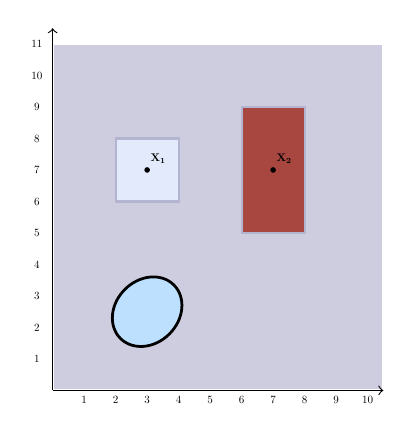
\begin{tikzpicture}[scale=0.4, transform shape]
				\draw[thick, fill=marine_blue!20, draw=white] (0,0) rectangle (10.5,11);
				% Draw the dendrogram
				\draw[-> ](0,0) -- (0,11.5);
				\draw[->] (0,0) -- (10.5,0);
				
			
				
				
			
			
				
			
				
				
				% Add distance labels
				\node at (1,-0.3) {$1$};
				\node at (2,-0.3) {$2$};
				\node at (3,-0.3) {$3$};
				\node at (4,-0.3) {$4$};
				\node at (5,-0.3) {$5$};
				\node at (6,-0.3) {$6$};
				\node at (7,-0.3) {$7$};
				\node at (8,-0.3) {$8$};
				\node at (9,-0.3) {$9$};
				\node at (10,-0.3) {$10$};
			
				\node at (-0.5,1) {1};
				\node at (-0.5,2) {2};
				\node at (-0.5,3) {3};
				\node at (-0.5,4) {4};
				\node at (-0.5,5) {5};
				\node at (-0.5,6) {6};
				\node at (-0.5,7) {7};
				\node at (-0.5,8) {8};
				\node at (-0.5,9) {9};
				\node at (-0.5,10) {10};
				\node at (-0.5,11) {11};
			
				% ellipse 
				\draw [rotate around={-45:(3,2.5)},line width=1pt, fill=ice_blue] (3,2.5) ellipse (1cm and 1.2cm);
				
				% rectangle 
				
				\draw[thick, fill=xdxdff, draw=marine_blue!30] (6,5) rectangle (8,9);
				\draw[thick, fill=grey_blue, draw=marine_blue!30] (2,6) rectangle (4,8);
				
			
				% Add points
			
				\draw [fill=black] (3,7) circle (2pt);
				\node at (3.35,7.35) {$\mathbf{X_1}$};
			
				\draw [fill=black] (7,7) circle (2pt);
				\node at (7.35,7.35) {$\mathbf{X_2}$};
			
				
				\end{tikzpicture}
		\end{column}
		\begin{column}{0.55\textwidth}
			\[c(x,y) = \frac{1}{2}\| x-y\|^2 + \sum_i v_i \|y-X_i\|^2\]
		\end{column}
	\end{columns}
\end{frame}
\begin{frame}
	\frametitle{Méthode gloutonne}
	\framesubtitle{Premier test : problème de séparation du nuage}
	On a le premier test suivant : 
	\begin{figure}[!htb]
			\centering 
			\begin{subfigure}{0.25\textwidth}
				\centering 
				\includegraphics[width=2.85cm]{images/nuage_divisible_1.png}
			\end{subfigure}
			\hspace*{\fill}
			\begin{subfigure}{0.25\textwidth}
				\centering 
				\includegraphics[width=3cm]{images/nuage_divisible_2.png}
			\end{subfigure}
			\hspace*{\fill}
			\begin{subfigure}{0.25\textwidth}
				\centering 
				\includegraphics[width=3cm]{images/nuage_divisible_3.png}
			\end{subfigure}
			\hspace*{\fill}
			
		\end{figure}
		\begin{figure}[!htb]

			\centering 
			\hspace*{\fill}
			\begin{subfigure}{0.25\textwidth}
				\centering 
				\includegraphics[width=3cm]{images/nuage_divisible_4.png}
			\end{subfigure}
			\hspace*{\fill}
			\begin{subfigure}{0.25\textwidth}
				\centering 
				\includegraphics[width=3cm]{images/nuage_divisible_5.png}
			\end{subfigure}
			\hspace*{\fill}
		\end{figure}
\end{frame}

\begin{frame}
	\frametitle{Méthode gloutonne}
	\framesubtitle{Premier test : problème de séparation du nuage}
	\emph{Correction du problème :} calculer l'écart moyen entre chaque points voisins et faire en sorte qu'il n'y ait aucun écart significativement plus grand que la moyenne.
	\begin{figure}
		\centering 
		\includegraphics[width=4cm]{images/nuage_divisible_3.png}
		\caption{Exemple de situation à éviter.}
	\end{figure}
\end{frame}


\begin{frame}
	\frametitle{Méthode gloutonne}
	\framesubtitle{Deuxième test : problème de densité}
	On a le second test suivant : 
	\begin{figure}[!htb]
			\centering 
			\begin{subfigure}{0.25\textwidth}
				\centering 
				\includegraphics[width=2.9cm]{images/nuage_densite_1.png}
			\end{subfigure}
			\hspace*{\fill}
			\begin{subfigure}{0.25\textwidth}
				\centering 
				\includegraphics[width=3cm]{images/nuage_densite_2.png}
			\end{subfigure}
			\hspace*{\fill}
			\begin{subfigure}{0.25\textwidth}
				\centering 
				\includegraphics[width=3cm]{images/nuage_densite_3.png}
			\end{subfigure}
			\hspace*{\fill}
			
		\end{figure}
		\begin{figure}[!htb]

			\centering 
			\hspace*{\fill}
			\begin{subfigure}{0.25\textwidth}
				\centering 
				\includegraphics[width=3cm]{images/nuage_densite_4.png}
			\end{subfigure}
			\hspace*{\fill}
			\begin{subfigure}{0.25\textwidth}
				\centering 
				\includegraphics[width=3cm]{images/nuage_densite_5.png}
			\end{subfigure}
			\hspace*{\fill}
		\end{figure}
\end{frame}

\begin{frame}
	\frametitle{Méthode gloutonne}
	\framesubtitle{Deuxième test : problème de densité}
	\emph{Correction du problème :} Calculer la densité initiale $d_0$ et l'écart autorisé $\varepsilon_d > 0$ à cette densité  pour qu'à chaque instant de la transition : \[d \in [d_0 - \varepsilon_d , d_0 + \varepsilon_d] \]
	\begin{figure}[!htb]
			\centering 
			\begin{subfigure}{0.25\textwidth}
				\centering 
				\includegraphics[width=2.9cm]{images/nuage_densite_corr_1.png}
			\end{subfigure}
			\hspace*{\fill}
			\begin{subfigure}{0.25\textwidth}
				\centering 
				\includegraphics[width=3cm]{images/nuage_densite_corr_2.png}
			\end{subfigure}
			\hspace*{\fill}
			\begin{subfigure}{0.25\textwidth}
				\centering 
				\includegraphics[width=3cm]{images/nuage_densite_corr_3.png}
			\end{subfigure}
			\hspace*{\fill}
			
		\end{figure}
\end{frame}
\begin{frame}
	\frametitle{Méthode gloutonne}
	\framesubtitle{Troisième test : dans des conditions plus compliquées}
	\begin{figure}[!htb]
			\centering 
			\begin{subfigure}{0.25\textwidth}
				\centering 
				\includegraphics[width=3cm]{images/nuage_final_1.png}
			\end{subfigure}
			\hspace*{\fill}
			\begin{subfigure}{0.25\textwidth}
				\centering 
				\includegraphics[width=3cm]{images/nuage_final_2.png}
			\end{subfigure}
			\hspace*{\fill}
			\begin{subfigure}{0.25\textwidth}
				\centering 
				\includegraphics[width=3cm]{images/nuage_final_3.png}
			\end{subfigure}
			\hspace*{\fill}
			
		\end{figure}
		\begin{figure}[!htb]

			\centering 
			\hspace*{\fill}
			\begin{subfigure}{0.25\textwidth}
				\centering 
				\includegraphics[width=3cm]{images/nuage_final_4.png}
			\end{subfigure}
			\hspace*{\fill}
			\begin{subfigure}{0.25\textwidth}
				\centering 
				\includegraphics[width=3cm]{images/nuage_final_5.png}
			\end{subfigure}
			\hspace*{\fill}
		\end{figure}
\end{frame}

\begin{frame}
	\frametitle{Méthode gloutonne}
	\framesubtitle{Conservation de la masse}
	Conservation de la masse entre une forme $A$ et une forme $B$ du nuage : \[\int_E \mu(x) dx = \boxed{\int_A \mu(x)dx =1 = \int_B \nu(x)dx} = \int_E \nu(x) dx\]
	Hypothèse forte : répartition uniforme de la matière\footnote{cas d'une sous-surface}, 
	\begin{figure}[h!]
		\centering 
		\includegraphics[width=5cm]{images/katrina.png}
		\caption{Ouragan Katrina, \emph{Fox 8}}
	\end{figure}
\end{frame}
\begin{frame}
	\frametitle{Méthode gloutonne}
	\framesubtitle{Conservation de la masse}
	Si $x \in A$,
	\[\mu(x) = \text{ cte } = \frac{1}{\mathcal{A}(A)}\]
	\begin{flushright}
		où $\mathcal{A}(A)$ est l'aire décrite par $A$.
	\end{flushright}
	Sinon, 
	\[\mu(x) = \text{ cte } = 0 \]
\end{frame}


\begin{frame}
	\frametitle{Méthode gloutonne}
	\framesubtitle{Calcul de l'aire d'un nuage : méthode de Monte-Carlo}
	On utilise pour cela la méthode de \emph{Monte Carlo} : \begin{figure}[h!]
		\centering 
		\includegraphics[width=4cm]{images/monte_carlo_cercle.png}
	\end{figure}
	À l'aide d'une loi uniforme, on lance $N$ points sur une surface $S$ comprenant notre nuage, on récupère alors le pourcentage $p$ de points dans le nuage, l'aire du nuage est donc approximativement de $p \times S$. 
\end{frame}

\begin{frame}
	\frametitle{Méthode gloutonne}
	\framesubtitle{Calcul de l'aire d'un nuage : méthode de Monte-Carlo}
	Appartenance au nuage : 
	\begin{figure}[!htb]
		\centering
		\begin{subfigure}{0.4\textwidth}
			\centering
			\includegraphics[width=4cm]{images/nuage_monte_carlo_0.jpeg}
			\caption{Point dans le nuage.}
		\end{subfigure}
		\hspace*{\fill}
		\begin{subfigure}{0.4\textwidth}
			\centering 
			\includegraphics[width=4.5cm]{images/nuage_monte_carlo_1.jpeg}
			\caption{Calcul d'appartenance.}
		\end{subfigure}
	\end{figure}
	\begin{flushright}
		$\Rightarrow$ Calcul en \underline{temps constant} : $\mathcal{O}(1)$.
	\end{flushright}
\end{frame}
\begin{frame}
	\frametitle{Méthode gloutonne}
	\framesubtitle{Calcul de l'aire d'un nuage : méthode de Monte-Carlo}
	\begin{figure}[h!]
		\centering 
		\hspace*{\fill}
		\begin{subfigure}{0.25\textwidth}
			\centering 
			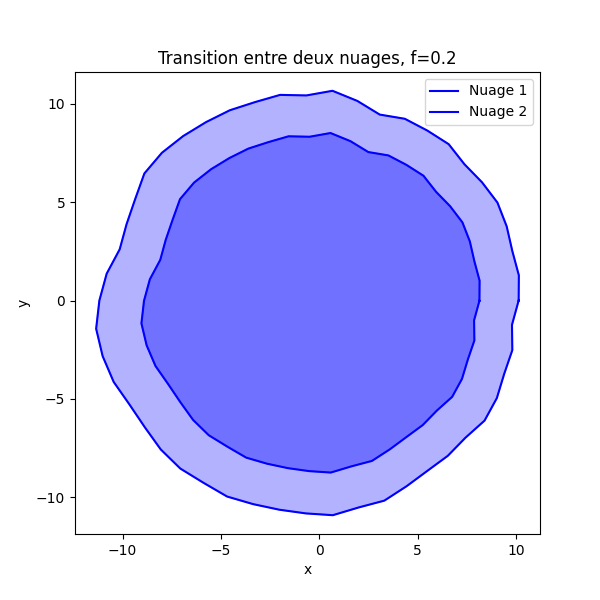
\includegraphics[width=3cm]{/Users/sacss/Desktop/Prépa/6.TIPE/khûbe/xp/contract_bary_f_0_2.png}
		\end{subfigure}
		\hspace*{\fill}
		\begin{subfigure}{0.25\textwidth}
			\centering 
			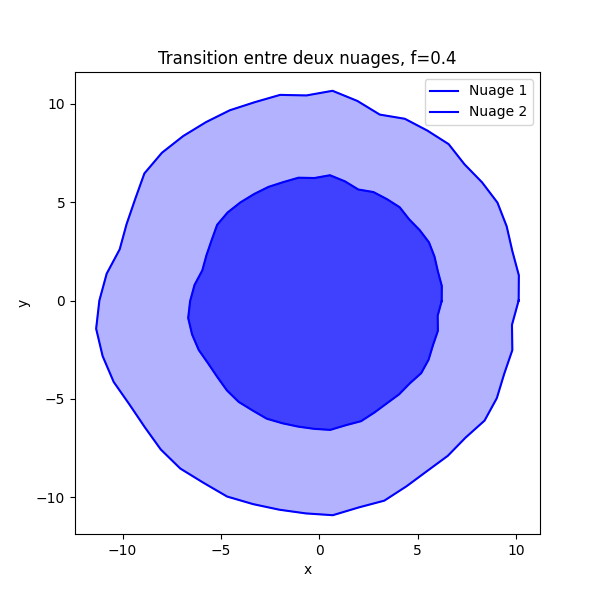
\includegraphics[width=3cm]{/Users/sacss/Desktop/Prépa/6.TIPE/khûbe/xp/contract_bary_f_0_4.png}
		\end{subfigure}
		\hspace*{\fill}
		\begin{subfigure}{0.25\textwidth}
			\centering 
			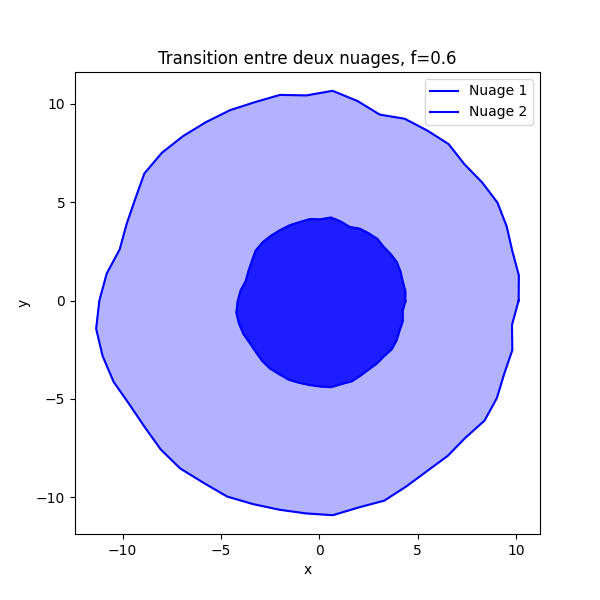
\includegraphics[width=3cm]{/Users/sacss/Desktop/Prépa/6.TIPE/khûbe/xp/contract_bary_f_0_6.png}
		\end{subfigure}
		\hspace*{\fill}
		
	\end{figure}


	\begin{figure}[h!]
		\centering 
		\hspace*{\fill}
		\begin{subfigure}{0.25\textwidth}
			\centering 
			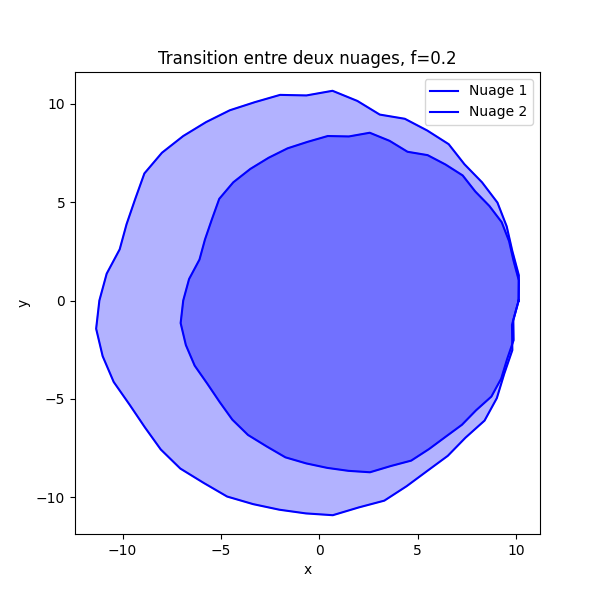
\includegraphics[width=3cm]{/Users/sacss/Desktop/Prépa/6.TIPE/khûbe/xp/contract_f_0_2.png}
		\end{subfigure}
		\hspace*{\fill}
		\begin{subfigure}{0.25\textwidth}
			\centering 
			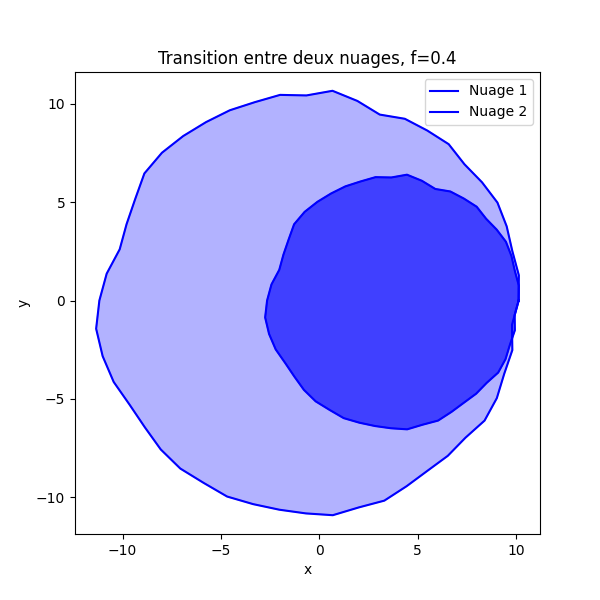
\includegraphics[width=3cm]{/Users/sacss/Desktop/Prépa/6.TIPE/khûbe/xp/contract_f_0_4.png}
		\end{subfigure}
		\hspace*{\fill}
		\begin{subfigure}{0.25\textwidth}
			\centering 
			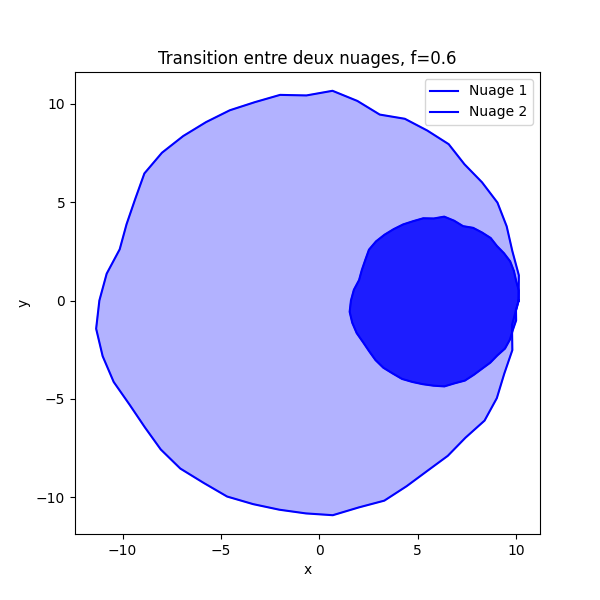
\includegraphics[width=3cm]{/Users/sacss/Desktop/Prépa/6.TIPE/khûbe/xp/contract_f_0_6.png}
		\end{subfigure}
		\hspace*{\fill}
		
	\end{figure}
\end{frame}
\begin{frame}
	\frametitle{Méthode gloutonne}
	\framesubtitle{Calcul de l'aire d'un nuage : méthode de Monte-Carlo}
	Complexité : \[\mathcal{O}(N)\]
	\begin{flushright}
		avec $N$ le nombre de points utilisés.
	\end{flushright}
	Pour le nuage de la figure~\ref{fig:nuage_python}, avec $ 3000 $ points : 
	\begin{center}
		\begin{tabular}{c|c}
		Aire estimée ($\text{m}^2$) & Temps requis (s) \\ \hline \hline 
		289.06 & 0.0816 \\ 
		289.58 & 0.0799 \\ 
		288.61 & 0.0783 \\
		289.35 & 0.0781 \\
		289.22 & 0.0780 \\
	\end{tabular}
	\end{center}
	\begin{flushright}
		\small $\Rightarrow$ Moins d'un dixième de seconde pour calculer l'aire.
	\end{flushright}
\end{frame}


\begin{frame}
	\frametitle{Méthode gloutonne}
	\framesubtitle{Conclusion}
	\begin{figure}[!htb]
			\centering 
			\begin{subfigure}{0.25\textwidth}
				\centering 
				\includegraphics[width=2.9cm]{images/ccl_1.png}
			\end{subfigure}
			\hspace*{\fill}
			\begin{subfigure}{0.25\textwidth}
				\centering 
				\includegraphics[width=3cm]{images/ccl_2.png}
			\end{subfigure}
			\hspace*{\fill}
			\begin{subfigure}{0.25\textwidth}
				\centering 
				\includegraphics[width=3cm]{images/ccl_3.png}
			\end{subfigure}
			\hspace*{\fill}
			
		\end{figure}
		\begin{figure}[!htb]

			\centering 
			\hspace*{\fill}
			\begin{subfigure}{0.25\textwidth}
				\centering 
				\includegraphics[width=3cm]{images/ccl_4.png}
			\end{subfigure}
			\hspace*{\fill}
			\begin{subfigure}{0.25\textwidth}
				\centering 
				\includegraphics[width=3cm]{images/ccl_5.png}
			\end{subfigure}
			\hspace*{\fill}
		\end{figure}
\end{frame}






\end{document}

